\documentclass{article}

% Useful packages
\usepackage{multicol}
\setlength{\columnsep}{1cm}

% Set page size and margins
% Replace `letterpaper' with `a4paper' for UK/EU standard size
\usepackage[a4paper,top=2cm,bottom=2cm,left=2cm,right=2cm,marginparwidth=1.75cm]{geometry}

\usepackage{caption}
\usepackage{amsmath}
\usepackage{siunitx}
\usepackage{wrapfig}
\usepackage{float}
\usepackage{graphicx}
\graphicspath{{images/}}
\usepackage{subcaption}
\usepackage[colorlinks=true, allcolors=blue]{hyperref}
\usepackage{xcolor}
\usepackage{listings}
\usepackage{import}
\usepackage{xcolor}

% Definieer de kleuren voor syntax highlighting
\definecolor{codegreen}{rgb}{0,0.6,0}
\definecolor{codegray}{rgb}{0.5,0.5,0.5}
\definecolor{codepurple}{rgb}{0.58,0,0.82}
\definecolor{backcolour}{rgb}{0.95,0.95,0.92}

\lstdefinestyle{mystyle}{
    backgroundcolor=\color{backcolour},
    commentstyle=\color{codegreen},
    keywordstyle=\color{codepurple},
    numberstyle=\tiny\color{codegray},
    basicstyle=\footnotesize\ttfamily,
    breakatwhitespace=false,
    breaklines=true,
    captionpos=b,
    keepspaces=true,
    numbers=left,
    numbersep=5pt,
    showspaces=false,
    showstringspaces=false,
    showtabs=false,
    tabsize=2
}

\usepackage[dutch]{babel}% Language setting


\title{Aandrijftechniek Moonrover}

\author{
  Vollmuller, Michel\\
  1809572\\
  \texttt{michel.vollmuller@student.hu.nl}
  \and
  Willems, Tijmen\\
  1805057\\
  \texttt{tijmen.willems@student.hu.nl}
}

\begin{document}
\maketitle

\begin{abstract}
    Hier komt een mooie abstract
\end{abstract}

% \begin{multicols}{2}


\section{Last}

\begin{align*}
  \textbf{Moonrover}\\
  &\text{Gewicht :} & 6 \, \text{kg} \\
  &\text{formaat (lengte x breedte):} & 40x25 \, \text{cm}\\
  \textbf{Wielen}\\
  &\text{diameter wielen :} & 15 \, \text{cm}\\
  &\text{wrijvingscoefficient :} & 0.9 \, \\
  &\text{rolweerstandcoefficient :} & 0.1 \, \\
  &\text{Massatraagheid (J) :} & \text{$2.1 \cdot 10^{-3}$} \, \text{$kg \cdot m^{2}$}\\
  \textbf{Specificaties}\\
  &\text{topsnelhied vlakke grond :} & 2.1 \, \text{$m.s^{-1}$}\\
  &\text{versnelling vlakke grond :} & 0.7 \, \text{$m/s^{2}$}\\
  &\text{vertraging vlakke grond :} & 0.5 \, \text{$m/s^{2}$}\\
  &\text{max helling :} & 30 \, \text{degrees}
\end{align*}
\\
\textbf{Situatie Klimmend}

\begin{figure}[h]
  \centering
  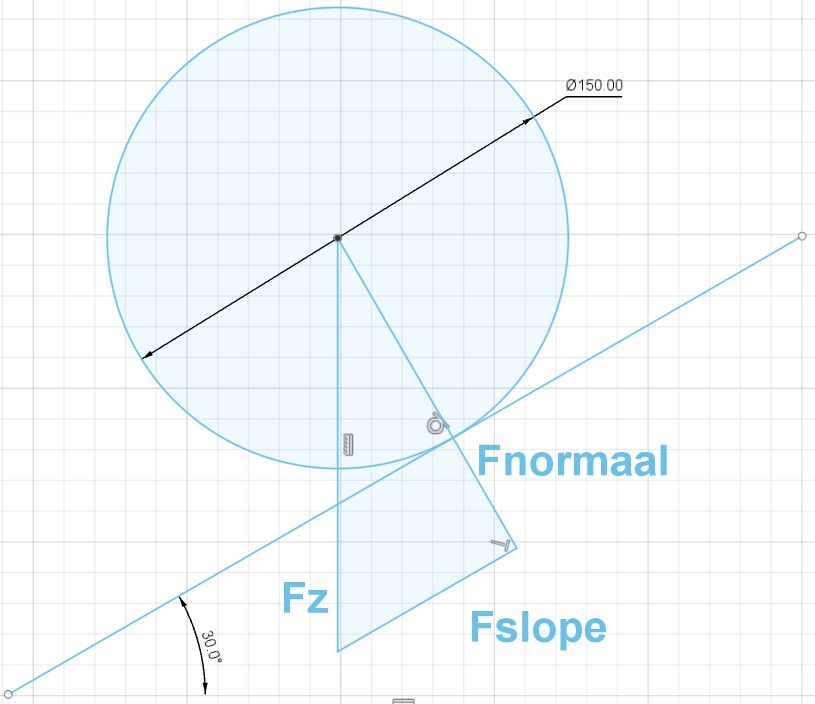
\includegraphics[scale=0.3]{last_helling.jpg}
  \caption{Last onder 30 graden helling}
\end{figure}
Gravitatieconstante van de maan is $g = 1.62$\\
Massa per wiel is $M = 1.5 kg$\\
$F_{z} = M \cdot g = 1.5 \cdot 1.62 = 2,43N$\\
$F_{normaal} = sin(60^\circ) \cdot F_{z} = 2.10$\\
$F_{slope} = cos(60^\circ) \cdot F_{z} = 1.215$\\
Kracht per wiel om stil te blijven staan is $T_{as} = F_{slope} \cdot r_{wiel} = 1,215 \cdot 0,075 = 0,09N$



% \end{multicols}

\section*{Conclusie}
Hier komt een mooie conclusie

%Bibliography
\bibliographystyle{IEEEtran}
\bibliography{bib}
\appendix

\end{document}